\documentclass[12pt]{article}

\usepackage[german]{babel}
\usepackage{amsmath}
\usepackage{amssymb} % to display symbols for real numbers, integers etc. Usage: \mathbb{R}
\usepackage{graphicx}
\usepackage{listings} % to display programming code
%\usepackage[ngerman]{babel}
\usepackage{color}
\usepackage{relsize} % to display scaled math symbols (big summation symbol etc.)
\usepackage{textcomp}

\DeclareGraphicsExtensions{.pdf,.jpeg,.png}
\definecolor{listinggray}{gray}{0.9}
\definecolor{lbcolor}{rgb}{0.9,0.9,0.9}
\lstset{ % to display programming code in nice colors
	backgroundcolor=\color{lbcolor},
	tabsize=4,
	rulecolor=,
	language=matlab,
		basicstyle=\scriptsize, %for extra small font size
        upquote=true,
        aboveskip={1.5\baselineskip},
        columns=fixed,
        showstringspaces=false,
        extendedchars=true,
        breaklines=true,
        prebreak = \raisebox{0ex}[0ex][0ex]{\ensuremath{\hookleftarrow}},
		frame=single, %draw frame
        showtabs=false,
        showspaces=false,
        showstringspaces=false,
        identifierstyle=\ttfamily,
        keywordstyle=\color[rgb]{0,0,1},
        commentstyle=\color[rgb]{0.133,0.545,0.133},
        stringstyle=\color[rgb]{0.627,0.126,0.941},
        numbers=left,
        stepnumber=1,
        firstnumber=1,
        numberfirstline=true,
        linewidth=14cm,
}

\title{\"Ubungsblatt 8\\ \glqq Mustererkennung\grqq}
\author{J. Cavojska, N. Lehmann, R. Toudic}
\date{28.06.2015}
\begin{document}
\maketitle
%\renewcommand{\contentsname}{Table of Contents}
\tableofcontents
\newpage

\section{Aufgabe 1 - Boolesche Funktionen und Perceptrons}

\subsection{1 a) Funktion zur Klassifizierung von Booleschen Funktionen}
\subsubsection{Code}
Hauptdatei: \textit{hw08.m}
\begin{lstlisting}[language=Matlab]
v1 = [0.3;0.5;-0.4];
v2 = [-0.8;-0.6;0.5];  
v3 = [0.7;0.6;-1];     

% signature: int classify_vec([float,float,float], {0|-1})
result_of_v1 = classify_vec(v1, 0)   % f10
result_of_v2 = classify_vec(v2, 0)   % f1
result_of_v3 = classify_vec(v3, 0)   % f8
\end{lstlisting}

Hilfsdatei: \textit{classify\_vec.m}
\begin{lstlisting}[language=Matlab]
function [y] = classify_vec(v, x)
if f0(v, x)
    y = 0;
elseif f1(v, x)
    y = 1;
elseif f2(v, x)
...
elseif f14(v, x)
    y = 14;
elseif f15(v, x)
    y = 15;
else
    y = 666;
end
\end{lstlisting}

Hilfsdatei: \textit{f0.m}
\begin{lstlisting}[language=Matlab]
% f00*2^0 + f01*2^1 + f10*2^2 + f11*2^3 = 0
function [y] = f0(v, x)
f00 = x*v(1) + x*v(2) + v(3) < 0;
f01 = x*v(1) + 1*v(2) + v(3) < 0;
f10 = 1*v(1) + x*v(2) + v(3) < 0;
f11 = 1*v(1) + 1*v(2) + v(3) < 0;
if f00 && f01 && f10 && f11
    y = 1;
else
    y = 0;
end
\end{lstlisting}

Hilfsdatei: \textit{f1.m}
\begin{lstlisting}[language=Matlab]
% f00*2^0 + f01*2^1 + f10*2^2 + f11*2^3 = 1
function [y] = f1(v, x)
f00 = x*v(1) + x*v(2) + v(3) >= 0;
f01 = x*v(1) + 1*v(2) + v(3) < 0;
f10 = 1*v(1) + x*v(2) + v(3) < 0;
f11 = 1*v(1) + 1*v(2) + v(3) < 0;
if f00 && f01 && f10 && f11
    y = 1;
else
    y = 0;
end
\end{lstlisting}
Die Hilfsdateien \textit{f2.m} bis \textit{f15.m} sind analog aufgebaut.\\

\subsection{1 b) Gleichverteilte Punkte auf einer Einheitskugel}
\subsubsection{Code}
\begin{lstlisting}[language=Matlab]
% create a sphere
[X,Y,Z] = sphere(100);
x = [X(:); X(:); X(:)];
y = [Y(:); Y(:); Y(:)];
z = [Z(:); Z(:); Z(:)];

% plot
figure('NumberTitle','off','Name','DIE Kugel');
hold on
mesh(0.99*X,0.99*Y,0.99*Z)

title('Aufgabe 1b - DIE Kugel');
xlabel('X Koordinaten');
ylabel('Y Koordinaten');
zlabel('Z Koordinaten');
axis([-1.1 1.1 -1.1 1.1]);

% 10000 random vectors
rv = random_vec(10000);

% plot
scatter3(rv(:,1), rv(:,2), rv(:,3), '.', 'm');
\end{lstlisting}
\newpage
Hilfsdatei: \textit{random\_vec.m}
\begin{lstlisting}[language=Matlab]
function [rv] = random_vec(n)
rng(0,'twister');
rv = [];
for i = 1:n
    varX = 2*pi*rand();
    varY = acos(2*rand()-1);
    x = cos(varX) * sin(varY);
    y = sin(varX) * sin(varY);
    z = 1         * cos(varY);
    vec = [x y z];
    rv = vertcat(rv,vec);
end
\end{lstlisting}
\subsubsection{Bilder}
\begin{center}
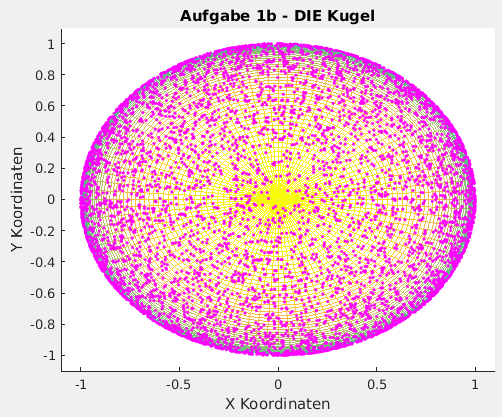
\includegraphics[width=10cm]{kugel01.png}
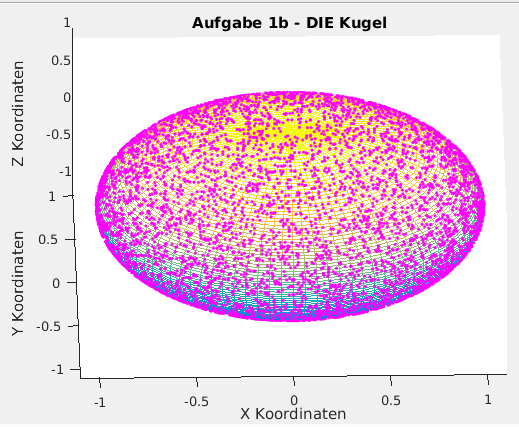
\includegraphics[width=10cm]{kugel02.png}
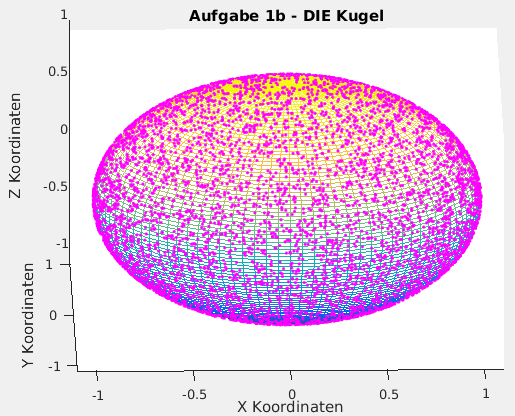
\includegraphics[width=10cm]{kugel03.png}
\end{center}
\subsection{1 c) Histogramm f\"ur Boolesche Funktionen mit 0, 1}
\subsubsection{Code}
\begin{lstlisting}[language=Matlab]
classifications1 = [];
for i = 1:10000
    v = rv(i,:);
    classifications1 = vertcat(classifications1, classify_vec(v, 0)); % classify v using 0, 1 as boolean values
end

% plot
figure('NumberTitle','off','Name','Histogram of Boolean Function Frequencies');
histogram(classifications1)

tabulate(classifications1)

frequencies = tabulate(classifications1);
maxfreq     = max(frequencies(:,2))
minfreq     = min(frequencies(:,2))
relation    = maxfreq / minfreq
\end{lstlisting}
\subsubsection{Resultate}
\begin{lstlisting}[language=Matlab]
Value    Count   Percent
  0     2730     27.30%
  1      429      4.29%
  2      318      3.18%
  3      488      4.88%
  4      362      3.62%
  5      491      4.91%
  7      148      1.48%
  8      149      1.49%
 10      485      4.85%
 11      331      3.31%
 12      479      4.79%
 13      384      3.84%
 14      413      4.13%
 15     2793     27.93%

maxfreq = 2793

minfreq = 148

relation = 18.8716
\end{lstlisting}
Histogramm:\\
\begin{center}
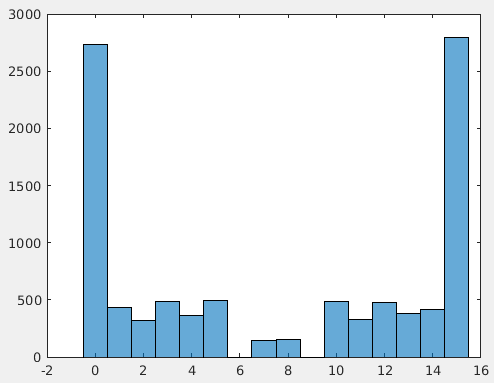
\includegraphics[width=10cm]{rel_freq_hist01.png}
\end{center}

\subsection{1 d) Histogramm f\"ur Boolesche Funktionen mit -1, 1}
\subsubsection{Code}
\begin{lstlisting}[language=Matlab]
classifications2 = [];
for i = 1:10000
    v = rv(i,:);
    classifications2 = vertcat(classifications2, classify_vec(v, -1));  % classify v using -1, 1 as boolean values
end

% plot
figure('NumberTitle','off','Name','Histogram of -1, 1 Boolean Frequencies');
histogram(classifications2)

tabulate(classifications2)

frequencies = tabulate(classifications2);
maxfreq     = max(frequencies(:,2))
minfreq     = min(frequencies(:,2))
relation    = maxfreq / minfreq
\end{lstlisting}
\subsubsection{Resultate}
\begin{lstlisting}[language=Matlab]
Value    Count   Percent
  0     1101     11.01%
  1      442      4.42%
  2      417      4.17%
  3     1067     10.67%
  4      381      3.81%
  5     1115     11.15%
  7      443      4.43%
  8      450      4.50%
 10     1047     10.47%
 11      442      4.42%
 12     1119     11.19%
 13      427      4.27%
 14      450      4.50%
 15     1099     10.99%

maxfreq = 1119

minfreq = 381

relation = 2.9370
\end{lstlisting}
\newpage
Histogramm:\\
\begin{center}
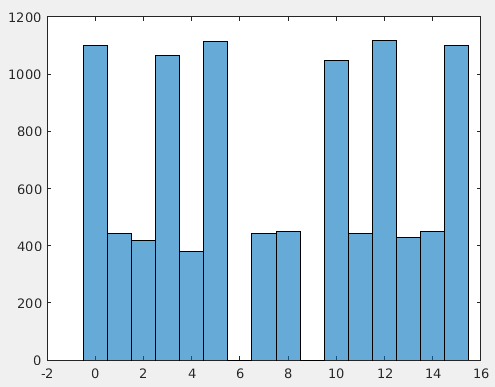
\includegraphics[width=10cm]{rel_freq_hist-11.png}
\end{center}

\end{document}